\subsection{Method Overview}
\label{sec:method_interface}

\method{} constructs compact training memories that carry graph information
and readable text across stages. This requires preserving relational
context before the current graph is released and coordinating numerical
feature construction with discrete text selection. We address these two
challenges through a learnable support matrix $Q$, where $Q_{ij}$ measures
the contribution of current node $i$ to new memory slot $j$. Each column
defines the source nodes from which a feature and its associated text are
constructed.

\autoref{fig:method_flow} summarizes three connected components.
\emph{Support learning} combines node features, neighborhood information,
and text semantics to initialize and refine $Q$
(\autoref{sec:method_support}).
\emph{Joint construction} converts this support into numerical features
and real texts, with a differentiable path for text feedback
(\autoref{sec:method_payload}).
\emph{Optimization and continual update} match the candidate memory to
current graph evidence and training signals, then append the resulting
block to the accumulated memory (\autoref{sec:method_update}).
Together, these components transfer current graph information into memory
features and allow training feedback from the selected texts to influence
their construction.

\begin{figure*}[t]
\centering
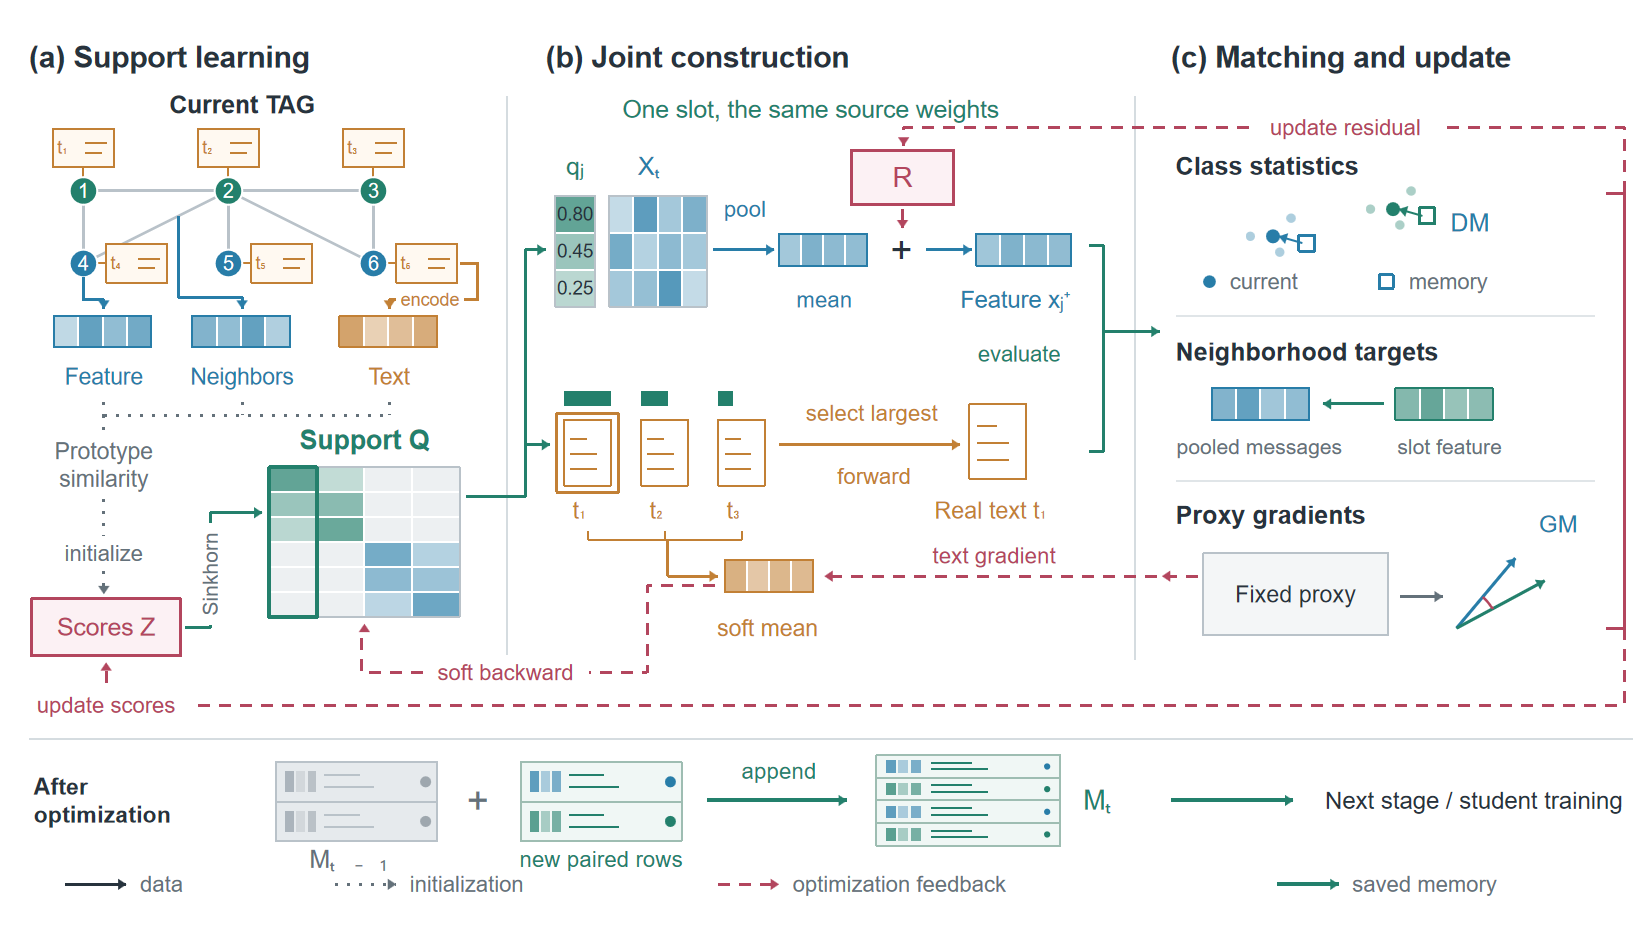
\includegraphics[width=\textwidth]{method_overview_final.png}
\caption{Overview of \method{}. (a) Node features, neighborhood context,
and attached texts from the current TAG initialize a balanced support matrix. (b) One slot and its
sources of the same class illustrate feature aggregation and real text selection
under $Q$. The soft text mean provides the backward path. (c) Class
statistics, neighborhood targets,
and proxy gradients guide construction. Proxy gradients use the same
accumulated memory on both sides. The optimized feature and text rows are
appended to memory for the next stage.}
\Description{Three panels show support learning, joint construction, and
matching. Each numbered node in the current TAG carries a corresponding text
attribute. Node features, neighborhoods, and encoded texts initialize scores.
A support matrix organized by class links nodes to slots.
One column supplies feature pooling and discrete document selection, with
a soft text representation for backpropagation. Comparisons with current
graph statistics and proxy training gradients update the support scores
and feature residual. A bottom strip shows old and new paired memory rows
being combined and passed to the next stage.}
\label{fig:method_flow}
\end{figure*}

\subsection{Learning Support from Graph and Text}
\label{sec:method_support}

The support matrix identifies which current nodes can jointly represent a
slot. Feature similarity alone describes individual attributes, whereas
neighboring nodes supply relational context and source texts supply
semantic content. We therefore describe each node using three normalized
views, comprising its numerical feature, a message aggregated from the normalized
features of its current neighbors, and the embedding of its cleaned text
from the frozen MiniLM encoder. Normalizing each view makes its similarity
depend on direction rather than vector magnitude.

At stage $t$, $Q$ has $n_t$ rows and $m_t$ columns, as defined in
\autoref{sec:memory_setting}. Within each
class, farthest-point selection on the combined representation provides
initial slot prototypes. Selecting points distant from the existing
prototypes spreads the starting slots across different regions of the
class. Let $\psi_i$ and $\pi_j$ denote the three views of node $i$ and
prototype $j$. Their initial support score is
\begin{equation}
 Z^0_{ij}=\operatorname{sim}(\psi_i,\pi_j),
 \qquad y_i=y_j .
\label{eq:method_init}
\end{equation}
Here $\operatorname{sim}$ is a weighted sum of cosine similarities of the
corresponding feature, neighborhood, and text views. The resulting
$Z^0$ initializes learnable scores $Z$. A class mask restricts each slot
to sources with its label, so the support has a block structure over
classes.

At each forward pass, we scale $Z$ by a temperature and apply Sinkhorn
normalization~\cite{sinkhorn} within each class block. Alternating row and
column normalization gives every node unit total mass and targets a mass
of $n_c/m_c$ for each slot in class $c$, where $n_c$ and $m_c$ are its
numbers of current nodes and slots. Iteration enforces these marginals
to numerical tolerance. This balancing distributes the class's support
across the available slots. Soft assignments let a source contribute to
several slots, while differentiability allows subsequent objectives to
refine those contributions. Thus, graph and text similarity provide the
starting organization, and memory construction supplies the signal for
learning it further.

\subsection{Joint Feature and Text Construction}
\label{sec:method_payload}

\textbf{Feature aggregation.}
For each slot, $Q$ defines a weighted set of source nodes. Let
$a_j=\sum_i Q_{ij}$ be its total support mass and let
$D_a=\operatorname{diag}(a_1,\ldots,a_{m_t})$. The feature branch computes
the corresponding weighted mean and adds a learnable residual,
\begin{equation}
 \bar X_t=D_a^{-1}Q^{\top}X_t,\qquad
 X_t^{+}=\bar X_t+R .
\label{eq:method_feature}
\end{equation}
Dividing by $a_j$ separates the scale of a feature from the number of
sources supporting it. Each pooled row is consequently a convex
combination of source features. The residual $R$ allows a local correction
beyond this average, which is useful when the subsequent graph and
training targets cannot be expressed by pooling alone. We initialize $R$
at zero and bound each row's norm relative to its current pooled feature
norm. The two variables have complementary roles. $Z$ changes which
sources contribute, while $R$ adjusts the resulting numerical feature.

\textbf{Text selection and feedback.}
The text branch selects the largest entry in the same column of $Q$,
giving source index $i_j^*$. The class mask ensures that the source and
slot share a label. The slot stores that source's
cleaned string $t_j^+=\bar t_{i_j^*}$. This gives the numerical mixture
and readable text a common source support. However, changing the scores
slightly may leave the selected index unchanged, preventing ordinary
backpropagation through the discrete choice. We therefore also form a
soft text mean. With $e_i$ denoting the normalized source embedding and
$\operatorname{Norm}$ denoting vector normalization, we use
\begin{equation}
\begin{aligned}
 \widetilde e_j
   &=\operatorname{Norm}\!\left(\frac{1}{a_j}\sum_i Q_{ij}e_i\right),\\
 e_j^{\mathrm{ST}}
   &=e_{i_j^*}+\widetilde e_j-\operatorname{sg}(\widetilde e_j).
\end{aligned}
\label{eq:method_text}
\end{equation}
The superscript ST denotes a straight-through estimator. The stop-gradient
operator $\operatorname{sg}$ preserves its input value
and stops its derivative. In the forward pass the soft terms cancel,
giving $e_j^{\mathrm{ST}}=e_{i_j^*}$, so the candidate is evaluated with
the real text it would store. In the backward pass the soft mean supplies
a surrogate derivative with respect to $Q$. With the text encoder fixed,
feedback changes the support scores. These changes modify
the feature mixture and can switch the selected text in a later forward
pass. In this way, text participates in construction through its training
signal as well as its initial similarity.

\subsection{Optimization and Continual Update}
\label{sec:method_objectives}
\label{sec:method_update}

The objectives guide the constructed rows through class
statistics, individual neighborhood representations, and the learning
signal of the student model.

\textbf{Retaining graph information.}
We first cache $H_t$, obtained by applying the symmetrically normalized
current adjacency with self-loops to $X_t$. Its row $h_i$ summarizes
the feature and neighborhood context of current node $i$.
For distribution matching (DM), we compare these messages with the candidate
features after nonlinear projections
$\phi_b(v)=\operatorname{Norm}(\operatorname{ReLU}(vW_b))$, where the
$B$ random matrices $W_b$ are fixed throughout construction and ReLU is the
rectified linear activation. Let $V_{t,c}$
and $S_{t,c}$ contain current nodes and new slots of class $c$,
respectively. We match their projected class means,
\begin{equation}
 L_{\mathrm{DM}}=\frac{1}{B}\sum_{b=1}^{B}\sum_{c\in\mathcal C_t}
 \left\|
 \frac{\sum_{i\in V_{t,c}}\phi_b(h_i)}{|V_{t,c}|}
 -\frac{\sum_{j\in S_{t,c}}\phi_b(x_j^+)}{|S_{t,c}|}
 \right\|_2^2 .
\label{eq:method_dm}
\end{equation}
Matching means in several nonlinear feature spaces constrains class
statistics beyond the original feature mean. Since the reference uses
propagated features, reducing this discrepancy transfers graph context
into the compact numerical representations.

Class means alone leave individual slots underconstrained. Propagation
matching therefore gives each slot a local target by pooling the rows of
$H_t$ with weights $Q_{ij}/a_j$ and normalizing the result. It penalizes
the angular discrepancy between this target and the normalized candidate
feature. The same source weights define both the feature mixture and its
neighborhood target. This term complements matching of class means by
retaining information about the
specific region represented by each slot.

\textbf{Retaining training signals.}
Feature statistics do not directly measure how a feature and its selected
text interact under the training objective. We therefore evaluate fixed
proxy models with the student's graph and text pairing loss and class
prompt supervision. For proxy $p$, let $g_p^{\mathrm{ref}}$ and
$g_p^{\mathrm{mem}}$ denote flattened parameter gradients evaluated on
the current increment and the candidate block, respectively, with
$M_{t-1}$ included on both sides. The accumulated memory thus supplies
the same historical training context for both gradients. We average
their direction and log magnitude discrepancies over $P$ proxy
initializations to define the gradient matching (GM) loss,
\begin{equation}
\begin{aligned}
 L_{\mathrm{GM}}=\frac{1}{P}\sum_{p=1}^{P}\bigg[&
 1-\cos(g_p^{\mathrm{ref}},g_p^{\mathrm{mem}})\\
 &+\frac{1}{4}\left|
 \log\frac{\|g_p^{\mathrm{ref}}\|_{\epsilon}}
               {\|g_p^{\mathrm{mem}}\|_{\epsilon}}
 \right|\bigg].
\end{aligned}
\label{eq:method_gm}
\end{equation}
Here $\|g\|_{\epsilon}=\max(\|g\|_2,\epsilon)$ safeguards norms near zero.
At fixed model parameters, a gradient determines a local
gradient descent update. Matching its
direction encourages a similar update direction, while the logarithmic norm
term controls relative differences in update magnitude. Differentiating
the candidate gradient with respect to the constructed data links this
objective to $Z$ and $R$. In particular, the pairing loss sends text
feedback through Eq.~\eqref{eq:method_text} to the support scores.

\textbf{Joint optimization and memory update.}
We combine the matching terms with support and feature regularization,
\begin{equation}
\begin{aligned}
 L={}&\lambda_{\mathrm{DM}}L_{\mathrm{DM}}
 +\lambda_{\mathrm{prop}}L_{\mathrm{prop}}
 +\lambda_{\mathrm{GM}}L_{\mathrm{GM}}\\
 &+\lambda_Q L_Q+\lambda_R L_R .
\end{aligned}
\label{eq:method_total}
\end{equation}
$L_Q$ is the mean squared deviation from the initial balanced support
$Q^0$, anchoring assignment learning to its initial source organization.
$L_R$ is the mean squared residual normalized by the initial pooled
feature norm, which controls the correction on a comparable relative
scale across slots. The coefficients balance the matching and
regularization terms and are fixed within a construction configuration.

Each iteration recomputes balanced support from $Z$, constructs the
feature and text branches, and evaluates the objective. Adam updates
$Z$ and $R$, after which the residual is projected back to its norm
bound. Current graph targets and reference gradients are cached for
reuse across these iterations. After optimization, we recompute the
features and selected texts and save them with their labels and source
identifiers as $M_t^+$. Appending this block gives
$M_t=M_{t-1}\oplus M_t^+$. Repeating the procedure makes features that
retain graph information and their associated texts available as training memory in
subsequent stages.
